\documentclass[a4paper,14pt]{extarticle}

\usepackage[T2A]{fontenc}			
\usepackage[utf8]{inputenc}			
\usepackage[english,russian]{babel}

\usepackage[
bookmarks=true, colorlinks=true, unicode=true,
urlcolor=black,linkcolor=black, anchorcolor=black,
citecolor=black, menucolor=black, filecolor=black,
]{hyperref}

\usepackage{color}
\usepackage{caption}
\DeclareCaptionFont{white}{\color{black}}
\DeclareCaptionFormat{listing}{\colorbox{white}{\parbox{\textwidth}{#1#2#3}}}
\captionsetup[lstlisting]{format=listing,labelfont=white,textfont=white}

\usepackage{amsmath,amsfonts,amssymb,amsthm,mathtools} 
\usepackage{wasysym}

%\usepackage[cache=false]{minted}

\usepackage{graphicx}
\usepackage{cmap}
\usepackage{indentfirst}

\usepackage{longtable}

\usepackage{listings} 
\usepackage{fancyvrb}

\usepackage{geometry}
\geometry{left=2cm}
\geometry{right=1.5cm}
\geometry{top=1cm}
\geometry{bottom=2cm}

\setlength{\parindent}{5ex}
\setlength{\parskip}{0.5em}

\usepackage{color}
\usepackage[cache=false, newfloat]{minted}
\newenvironment{code}{\captionsetup{type=listing}}{}
\SetupFloatingEnvironment{listing}{name=Листинг}
 
 
 \begin{document}
 	
 	\def\figurename{Рисунок}
 	
 	\begin{minipage}{0.2\textwidth}
 		
\includegraphics[scale=0.05]{img/bmstu.png}
 	\end{minipage}
 	\begin{minipage}{0.7\textwidth}
 		\small
 		\begin{center}
 			\textbf{Министерство науки и высшего образования Российской Федерации}
 			
 			\textbf{Федеральное государственное бюджетное образовательное учреждение высшего образования «Московский государственный технический университет имени Н.Э. Баумана}
 			
 			\textbf{(национальный исследовательский университет)»}
 			
 			\textbf{(МГТУ им. Н.Э. Баумана)}
 		\end{center}
 	\end{minipage}
 	
 	\vspace*{5mm}
 	
 	\normalsize
 	\begin{flushleft}
 		Факультет: <<Информатика и системы управления>>
 		
 		Кафедра: <<Программное обеспечение ЭВМ и информационные технологии>>
 	\end{flushleft}
 	
 	\vspace*{30mm}
 	
 	\LARGE
 	\begin{center}
 		\textbf{Расчетно-пояснительная записка}
 		
 		%	\textbf{к курсовому проекту на тему:}
 		\textbf{к курсовой работе на тему:}
 		
 		\textbf{<<Мониторинг вызовов функций ядра Linux>>}
 	\end{center}
 	
 	\vspace*{15mm}
 	
 	\large
 	\begin{flushleft}
 		\textbf{Студент:} Левушкин И. К. \\
 		\textbf{Группа:} ИУ7-72Б \\
 		%        \textbf{Оценка (баллы):} \\
 		\textbf{Научный руководитель:} Филиппов М.В.
 	\end{flushleft}
 	
 	\vspace*{50mm}
 	
 	\large
 	\begin{center}
 		Москва, 2020 г.
 	\end{center}
 	
 	\thispagestyle{empty}
 	
 	\newpage
 	
 	\tableofcontents
 	\newpage
 	\section*{Введение}
 	\addcontentsline{toc}{section}{Введение}
 	
 	Иногда, при работе с Linux-системами, требуется перехватывать вызовы важ­ных функций внутри ядра (вроде открытия файлов и запуска процессов) для обес­печения возможности мониторинга активности в системе или превентивного блоки­рования деятельности подозрительных процессов.
 	
 	Проект посвящен исследованию способов перехвата вызовов функций внут­ри ядра. Целью проекта является разработка подхода, позволяющего удобно перехватить любую функцию в ядре по имени и выполнить свой код вокруг её вызовов.
 	
 	\newpage
 	
 	\section{Аналитический раздел}
 	
 	В соответствии с заданием на курсовой проект необходимо разработать программное обеспечение, представляющее собой загружаемый модуль ядра Linux. Модуль ядра должен уметь перехватывать заданные события в системе, инициирующиеся средством исполнения экспортируемых функция ядра.
 	
 	Программное обеспечение должно обеспечивать перехват всех вызовов нужных функций и осуществлять вывод в буфер сообщений ядра информацию об адресе, по которому вызывается функция, ее параметрах и возвращаемом значении.
 	
 	\subsection{Анализ подходов реализации}
 	
 	\begin{itemize}
 		\item Linux Security API
 		\item Модификация таблицы системных вызовов
 		\item Использование kprobes
 		\item Сплайсинг
 		\item Ftrace
 	\end{itemize}
 
 	\subsubsection{Linux Security API}
 	
 	Наиболее правильным было бы использование Linux Security API — специального интерфейса, созданного именно для этих целей. В критических местах ядерного кода расположены вызовы security-функций, которые в свою очередь вызывают коллбеки, установленные security-модулем. Security-модуль может изучать контекст операции и принимать решение о её разрешении или запрете.
 	
 	К сожалению, у Linux Security API есть пара важных ограничений:
 	\begin{itemize}
 		\item security-модули не могут быть загружены динамически, являются частью ядра и требуют его пересборки
 		\item в системе может быть только один security-модуль (с небольшими исключениями)
 	\end{itemize}
 	
 	Если по поводу множественности модулей позиция разработчиков ядра неоднозначная, то запрет на динамическую загрузку принципиальный: security-модуль должен быть частью ядра, чтобы обеспечивать безопасность постоянно, с момента загрузки. Таким образом, для использования Security API необходимо поставлять собственную сборку ядра, а также интегрировать дополнительный модуль с SELinux или AppArmor, которые используются популярными дистрибутивами.
 	
 	\subsubsection{Модификация таблицы системных вызовов}
 	
 	Мониторинг требовался в основном для действий, выполняемых пользовательскими приложениями, так что в принципе мог бы быть реализован на уровне системных вызовов. Как известно, Linux хранит все обработчики системных вызовов в таблице sys\_call\_table. Подмена значений в этой таблице приводит к смене поведения всей системы. Таким образом, сохранив старое значения обработчика и подставив в таблицу собственный обработчик, мы можем перехватить любой системный вызов.
 	
 	У этого подхода есть определённые преимущества:
 	\begin{itemize}
 		\item Полный контроль над любыми системными вызовами — единственным интерфейсом к ядру у пользовательских приложений. Используя его мы можем быть уверены, что не пропустим какое-нибудь важное действие, выполняемое пользовательским процессом.
 		\item Минимальные накладные расходы. Есть единоразовые капитальные вложения при обновлении таблицы системных вызовов. Помимо неизбежной полезной нагрузки мониторинга, единственным расходом является лишний вызов функции (для вызова оригинального обработчика системного вызова).
 		\item Минимальные требования к ядру. При желании этот подход не требует каких-либо дополнительных конфигурационных опций в ядре, так что в теории поддерживает максимально широкий спектр систем.
 	\end{itemize}
 	
 	Однако, подход не лишен недостатков:
 	\begin{itemize}
 		\item Техническая сложность реализации. Сама по себе замена указателей в таблице не представляет трудностей. Но сопутствующие задачи требуют неочевидных решений и определённой квалификации:
 		\begin{itemize}
 			\item поиск таблицы системных вызовов
 			\item обход защиты от модификации таблицы
 			\item атомарное и безопасное выполнение замены
 		\end{itemize}
 		\item Невозможность перехвата некоторых обработчиков. В ядрах до версии 4.16 обработка системных вызовов для архитектуры x86\_64 содержала целый ряд оптимизаций. Некоторые из них требовали того, что обработчик системного вызова являлся специальным переходничком, реализованным на ассемблере. Соответственно, подобные обработчики порой сложно, а иногда и вовсе невозможно заменить на свои, написанные на Си. Более того, в разных версиях ядра используются разные оптимизации, что добавляет в копилку технических сложностей.
 		\item Перехватываются только системные вызовы. Этот подход позволяет заменять обработчики системных вызовов, что ограничивает точки входа только ими. Все дополнительные проверки выполняются либо в начале, либо в конце, и у нас есть лишь аргументы системного вызова и его возвращаемое значение. Иногда это приводит к необходимости дублировать проверки на адекватность аргументов и проверки доступа. Иногда вызывает лишние накладные расходы, когда требуется дважды копировать память пользовательского процесса: если аргумент передаётся через указатель, то его сначала придётся скопировать нам самим, затем оригинальный обработчик скопирует аргумент ещё раз для себя. Кроме того, в некоторых случаях системные вызовы предоставляют слишком низкую гранулярность событий, которые приходится дополнительно фильтровать от шума.
 	\end{itemize}
 	
 	Данный подход позволяет полностью подменить таблицу системных вызовов что является несомненным плюсом, но также ограничивает количество функций, которые можно мониторить.
 	
 	\subsubsection{Использование kprobes}
 	
 	Одним из вариантов, которые рассматривались, было использование kprobes: специализированного API, в первую очередь предназначенного для отладки и трассирования ядра. Этот интерфейс позволяет устанавливать пред- и постобработчики для любой инструкции в ядре, а также обработчики на вход и возврат из функции. Обработчики получают доступ к регистрам и могут их изменять. Таким образом, можно было бы получить как мониторинг, так и возможность влиять на дальнейший ход работы.
 	
 	Преимущества, которые даёт использование kprobes для перехвата:
 	\begin{itemize}
 		\item Зрелый API. Kprobes существуют и улучшаются с 2002 года. Они обладают хорошо задокументированным интерфейсом, большинство подводных камней уже найдено, их работа по возможности оптимизирована.
 		\item Перехват любого места в ядре. Kprobes реализуются с помощью точек останова (инструкции int3), внедряемых в исполнимый код ядра. Это позволяет устанавливать kprobes в буквально любом месте любой функции, если оно известно. Аналогично, kretprobes реализуются через подмену адреса возврата на стеке и позволяют перехватить возврат из любой функции (за исключением тех, которые управление в принципе не возвращают).
 	\end{itemize}
 	
 	Недостатки kprobes:
 	
 	\begin{itemize}
 		\item Техническая сложность. Kprobes — это только способ установить точку останова в любом места ядра. Для получения аргументов функции или значений локальных переменных надо знать, в каких регистрах или где на стеке они лежат, и самостоятельно их оттуда извлекать. Для блокировки вызова функции необходимо вручную модифицировать состояние процесса так, чтобы процессор подумал, что он уже вернул управление из функции.
 		\item Jprobes объявлены устаревшими. Jprobes — это надстройка над kprobes, позволяющая удобно перехватывать вызовы функций. Она самостоятельно извлечёт аргументы функции из регистров или стека и вызовет ваш обработчик, который должен иметь ту же сигнатуру, что и перехватываемая функция. Подвох в том, что jprobes объявлены устаревшими и вырезаны из современных ядер.
 		\item Нетривиальные накладные расходы. Расстановка точек останова дорогая, но она выполняется единоразово. Точки останова не влияют на остальные функции, однако их обработка относительно недешёвая. К счастью, для архитектуры x86\_64 реализована jump-оптимизация, существенно уменьшающая стоимость kprobes, но она всё ещё остаётся больше, чем, например, при модификации таблицы системных вызовов.
 		\item Ограничения kretprobes. Kretprobes реализуются через подмену адреса возврата на стеке. Соответственно, им необходимо где-то хранить оригинальный адрес, чтобы вернуться туда после обработки kretprobe. Адреса хранятся в буфере фиксированного размера. В случае его переполнения, когда в системе выполняется слишком много одновременных вызовов перехваченной функции, kretprobes будет пропускать срабатывания.
 		\item Отключенное вытеснение. Так как kprobes основывается на прерываниях и жонглирует регистрами процессора, то для синхронизации все обработчики выполняются с отключенным вытеснением (preemption). Это накладывает определённые ограничения на обработчики: в них нельзя ждать — выделять много памяти, заниматься вводом-выводом, спать в таймерах и семафорах, и прочие известные вещи.
 	\end{itemize}
 
 	\subsubsection{Сплайсинг}
 	
 	Классический способ перехвата функций, заключающийся в замене инструкций в начале функции на безусловный переход, ведущий в обработчик. Оригинальные инструкции переносятся в другое место и исполняются перед переходом обратно в перехваченную функцию. С помощью двух переходов вшивается (splice in) свой дополнительный код в функцию, поэтому такой подход называется сплайсингом.
 	
 	Именно таким образом и реализуется jump-оптимизация для kprobes. Используя сплайсинг можно добиться тех же результатов, но без дополнительных расходов на kprobes и с полным контролем ситуации.
 	
 	Преимущества сплайсинга:
 	\begin{itemize}
 		\item Минимальные требования к ядру. Сплайсинг не требует каких-либо особенных опций в ядре и работает в начале любой функции. Нужно только знать её адрес.
 		\item Минимальные накладные расходы. Два безусловных перехода — вот и все действия, которые надо выполнить перехваченному коду, чтобы передать управление обработчику и обратно. Подобные переходы отлично предсказываются процессором и являются очень дешёвыми.
 	\end{itemize}
 	
 	Недостатки:
 	\begin{itemize}
 		\item Техническая сложность. Она зашкаливает. Нельзя просто так взять и переписать машинный код. Вот краткий и неполный список задач, которые придётся решить:
 		\begin{itemize}
 			\item синхронизация установки и снятия перехвата (что если функцию вызовут прямо в процессе замены её инструкций?)
 			\item обход защиты на модификацию регионов памяти с кодом
 			\item инвалидация кешей процессора после замены инструкций
 			\item дизассемблирование заменяемых инструкций, чтобы скопировать их целыми
 			\item проверка на отсутствие переходов внутрь заменяемого куска
 			\item проверка на возможность переместить заменяемый кусок в другое место
 		\end{itemize}
 	\end{itemize}
 
 	\subsubsection{Ftrace}
 	
 	Ftrace — это фреймворк для трассирования ядра на уровне функций. Он разрабатывается с 2008 года и обладает удобным интерфейсом для пользовательских программ. Ftrace позволяет отслеживать частоту и длительность вызовов функций, отображать графы вызовов, фильтровать интересующие функции по шаблонам, и так далее.
 	
 	Реализуется ftrace на основе ключей компилятора -pg и -mfentry, которые вставляют в начало каждой функции вызов специальной трассировочной функции mcount() или \_\_fentry\_\_(). Обычно, в пользовательских программах эта возможность компилятора используется профилировщиками, чтобы отслеживать вызовы всех функций. Ядро же использует эти функции для реализации фреймворка ftrace.
 	
 	Вызывать ftrace из каждой функции — это, разумеется, не дёшево, поэтому для популярных архитектур доступна оптимизация: динамический ftrace. Суть в том, что ядро знает расположение всех вызовов mcount() или \_\_fentry\_\_() и на ранних этапах загрузки заменяет их машинный код на nop — специальную ничего не делающую инструкцию. При включении трассирования в нужные функции вызовы ftrace добавляются обратно. Таким образом, если ftrace не используется, то его влияние на систему минимально.
 	
 	Преимущества:
 	\begin{itemize}
 		\item Зрелый API и простой код. Использование готовых интерфейсов в ядре существенно упрощает код. Вся установка перехвата требует пары вызовов функций, заполнение двух полей в структуре. Остальной код — это исключительно бизнес-логика, выполняемая вокруг перехваченной функции.
 		\item Перехват любой функции по имени. Для указания интересующей нас функции достаточно написать её имя в обычной строке. Не требуются какие-то особые реверансы с редактором связей, разбор внутренних структур данных ядра, сканирование памяти, или что-то подобное. Можно перехватить любую функцию (даже не экспортируемую для модулей), зная лишь её имя.
 		\item Перехват совместим с трассировкой. Очевидно, что этот способ не конфликтует с ftrace, так что с ядра всё ещё можно снимать очень полезные показатели производительности. Использование kprobes или сплайсинга может помешать механизмам ftrace.
 	\end{itemize}
 	
 	Недостатки:
 	\begin{itemize}
 		\item Требования к конфигурации ядра. Для успешного выполнения перехвата функций с помощью ftrace ядро должно предоставлять целый ряд возможностей:
 		\begin{itemize}
 			\item список символов kallsyms для поиска функций по имени
 			\item фреймворк ftrace в целом для выполнения трассировки
 			\item опции ftrace, критически важные для перехвата
 		\end{itemize}
 	\end{itemize}
 	
 	Все эти возможности не являются критичными для функционирования системы и могут быть отключены в конфигурации ядра. Правда, обычно ядра, используемые популярными дистрибутивами, все эти опции в себе всё равно содержат, так как они не влияют на производительность и полезны при отладке. Однако, если вам необходимо поддерживать какие-то особенные ядра, то следует иметь в виду эти требования.
 	
 	\begin{itemize}
 		\item Накладные расходы на ftrace меньше, чем у kprobes (так как ftrace не использует точки останова), но они выше, чем у сплайсинга, сделанного вручную. Действительно, динамический ftrace, является сплайсингом, только вдобавок выполняющий код ftrace и другие коллбеки.
 		\item Оборачиваются функции целиком. Как и традиционный сплайсинг, данный подход полностью оборачивает вызовы функций. Однако, если сплайсинг технически возможно выполнить в любом месте функции, то ftrace срабатывает исключительно при входе. Естественно, обычно это не вызывает сложностей и даже наоборот удобно, но подобное ограничение иногда может быть недостатком.
 	\end{itemize}
 
 	\subsection{Загружаемые модули ядра Linux }
 	Ядро Linux относится к категории так называемых монолитных – это означает, что большая часть функциональности операционной системы называется ядром и запускается в привилегированном режиме. Этот подход отличен от подхода микроядра, когда в режиме ядра выполняется только основная функциональность (взаимодействие между процессами [inter-process communication, IPC], диспетчеризация, базовый ввод-вывод [I/O], управление памятью), а остальная функциональность вытесняется за пределы привилегированной зоны (драйверы, сетевой стек, файловые системы). Можно было бы подумать, что ядро Linux очень статично, но на самом деле все как раз наоборот.
 	Ядро Linux динамически изменяемое – это означает, что вы можете загружать в ядро дополнительную функциональность, выгружать функции из ядра и даже добавлять новые модули, использующие другие модули ядра. Преимущество загружаемых модулей заключается в возможности сократить расход памяти для ядра, загружая только необходимые модули (это может оказаться важным для встроенных систем).
 	
 	Linux – не единственное (и не первое) динамически изменяемое монолитное ядро. Загружаемые модули поддерживаются в BSD-системах, Sun Solaris, в ядрах более старых операционных систем, таких как OpenVMS, а также в других популярных ОС, таких как Microsoft Windows и Apple Mac OS X.
 	
 	\subsubsection{Устройство модуля ядра}
 	Загружаемые модули ядра имеют ряд фундаментальных отличий от элементов, интегрированных непосредственно в ядро, а также от обычных программ. Обычная программа содержит главную процедуру (main)в отличие от загружаемого модуля, содержащего функции входа и выхода (в версии 2.6 эти функции можно именовать как угодно). Функция входа вызывается, когда модуль загружается в ядро, а функция выхода – соответственно при выгрузке из ядра. Поскольку функции входа и выхода являются пользовательскими, для указания назначения этих функций используются макросы module\_init и module\_exit . Загружаемый модуль содержит также набор обязательных и дополнительных макросов. Они определяют тип лицензии, автора и описание модуля, а также другие параметры. Пример очень простого загружаемого модуля приведен на рисунке  \ref{fig:an01} .
 	\begin{figure}[h!]
 		\centering
 		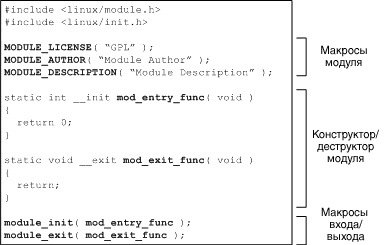
\includegraphics[width=0.6\textwidth]{img/1.png}
 		\caption{Пример загружаемого модуля с разделами ELF}
 		\label{fig:an01}
 	\end{figure}
 
 \subsection*{Выводы по аналитическому разделу}
 
 Проанализировав все изученные подходы к реализации мониторинга за вызовами функций ядра, был выбран подход с ftrace, поскольку он обладает рядом преимуществ по сравнению с другими подходами, такими как, простота написания кода за счет использования зрелого API, а также возможность перехватывать функцию по ее имени.
 
 \newpage
 
 \section{Конструкторский раздел}
 
 \subsection{Структура программного обеспечения}
 
 В состав программного обеспечения входит только загружаемый модуль яд­ра, следящий за вызовом нужных функций - sys\_execve и sys\_clone, с последующим выводом информации о них в буфер сообщений ядра.
 
 \subsection{Перехват функций}
 
 Каждую перехватываемую функцию можно описать следующей структурой:
 
 \begin{listing}[h]
 	\caption{ftrace\_hook}
 	\begin{minted}[frame=single,linenos,framerule=2pt, fontsize=\footnotesize]{C++}
 	/**
 	* struct ftrace_hook - описывает перехватываемую функцию
 	*
 	* @name:       имя перехватываемой функции
 	*
 	* @function:   адрес функции-обёртки, которая будет вызываться вместо
 	*              перехваченной функции
 	*
 	* @original:   указатель на место, куда следует записать адрес
 	*              перехватываемой функции, заполняется при установке
 	*
 	* @address:    адрес перехватываемой функции, выясняется при установке
 	*
 	* @ops:        служебная информация ftrace, инициализируется нулями,
 	*              при установке перехвата будет доинициализирована
 	*/
 	struct ftrace_hook {
	 	const char *name;
	 	void *function;
	 	void *original;
	 	
	 	unsigned long address;
	 	struct ftrace_ops ops;
 	};
 	\end{minted}
 \end{listing}
 
 Пользователю необходимо заполнить только первые три поля: name, function, original. Остальные поля считаются деталью реализации. Описание всех перехватываемых функций можно собрать в массив и использовать макросы, чтобы повысить компактность кода:
 
 \begin{listing}[h]
 	\caption{ftrace\_hook define}
 	\begin{minted}[frame=single,linenos, framerule=2pt, fontsize=\footnotesize]{C++}
 	 #define HOOK(_name, _function, _original)       
 	{                                       
	 	.name = (_name),                    
	 	.function = (_function),            
	 	.original = (_original),            
 	}
 	
 	static struct ftrace_hook hooked_functions[] = {
	 	HOOK("sys_clone",   fh_sys_clone,   &real_sys_clone),
	 	HOOK("sys_execve", fh_sys_execve, &real_sys_execve),
 	};
 	\end{minted}
\end{listing}
 
 \subsection{Схема работы перехвата}
 
 Рассмотрим пример: терминале набирается команда ls, чтобы увидеть список файлов в текущей директории. Командный интерпретатор для запуска нового процесса использует пару функций fork() + execve() из стандартной библиотеки языка Си. Внутри эти функции реализуются через системные вызовы clone() и execve() соответственно. Допустим, мы перехватываем системный вызов execve(), чтобы контролировать запуск новых процессов.
 
 \newpage
 
 В графическом виде перехват функции-обработчика выглядит так:
 \begin{figure}[h!]
 	\centering
 	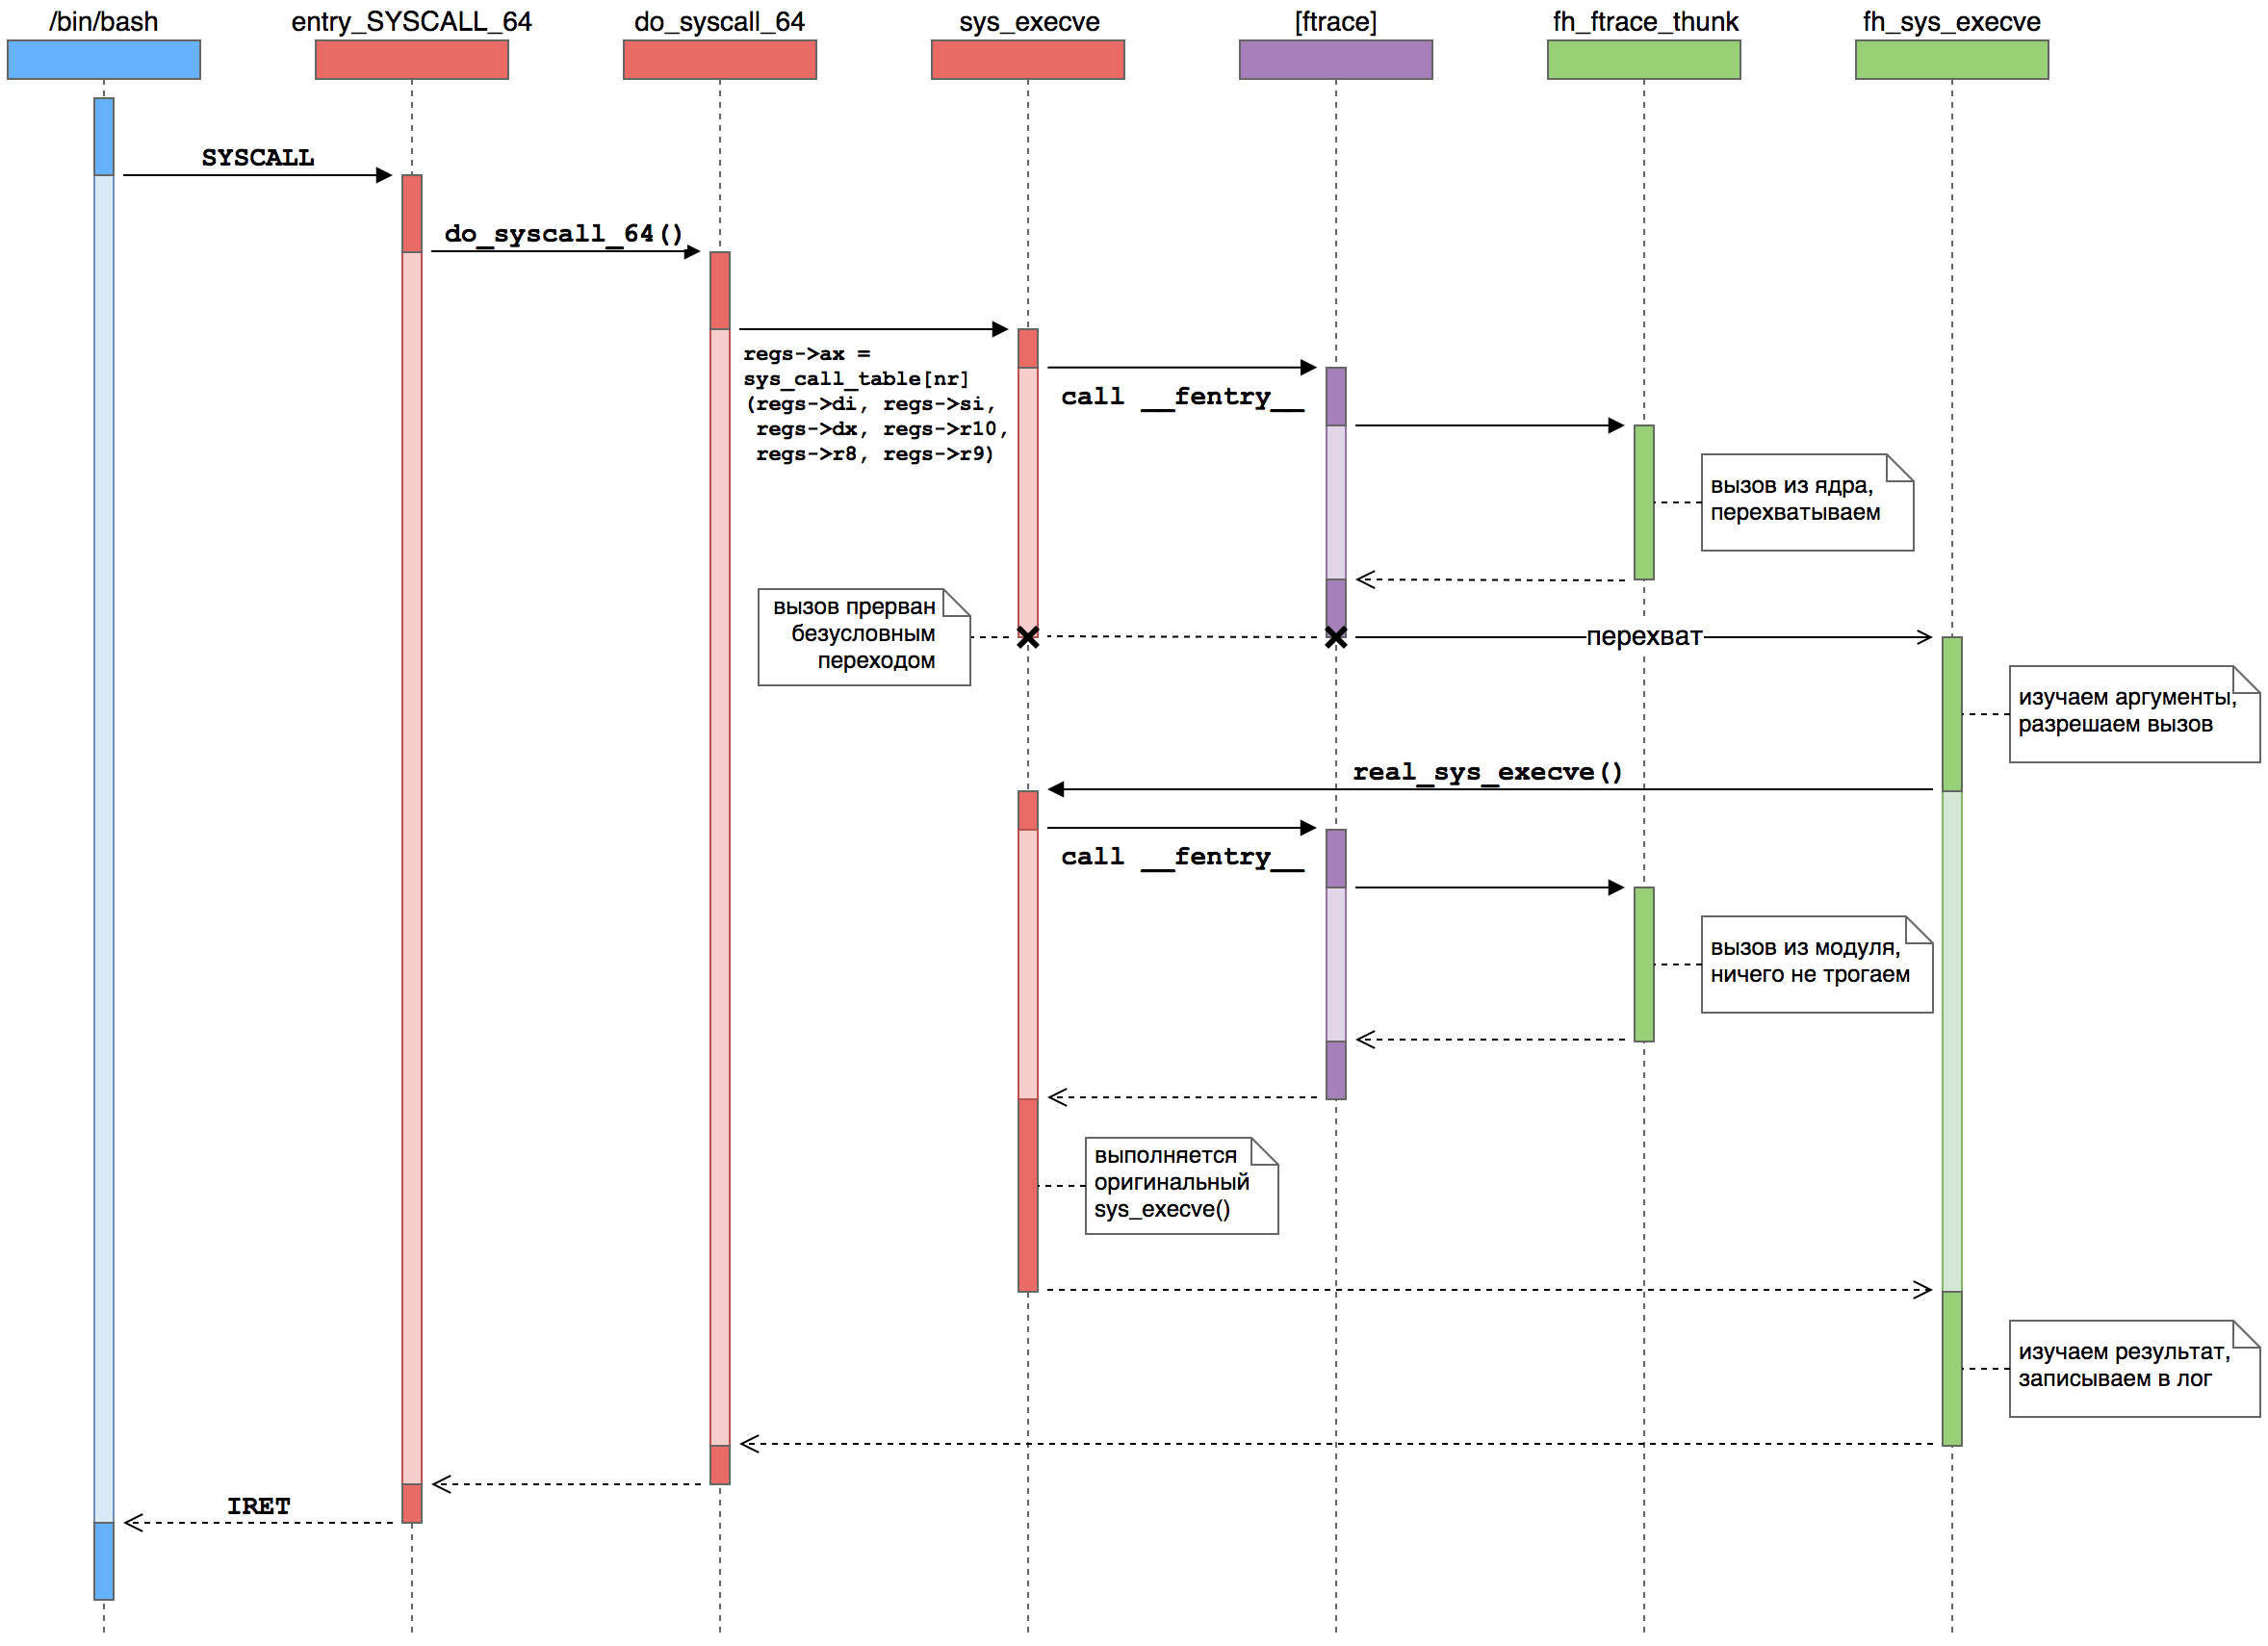
\includegraphics[width=1.0\textwidth]{img/hook_work_scheme.png}
 	\caption{Алгоритм работы функции-перехватчика}
 	\label{fig:spire00}
 \end{figure}
 
 \newpage
 
 \section{Технологический раздел}
 
 \subsection{Выбор языка программирования}
 
 Для реализации загружаемого модуля был выбран язык С с использованием встроенного в ОС Linux компилятора GCC. Выбор языка основан на том, что исходный код ядра, предо­ставляемый системой, написан на С, и использование другого языка программиро­вания в данном случае было бы нецелесообразным.

\subsection{Выбор среды разработки}
 
 Для написания программы, был выбран текстовый редактор Sublime text 3.
 \begin{itemize}
 	\item Огромное количество плагинов, которые позволяют делать работу быстрее
 	\item Возможность гибкой настройки под себя
 	\item Много встроенных команд и комбинаций
 \end{itemize}

\subsection{Модуль ядра}

\subsubsection{Обертки перехватываемых функций}

Обёртки над перехватываемыми функциями выглядят следующим образом:

\newpage

\begin{listing}[h]
	\caption{fh\_sys\_clone}
	\begin{minted}[frame=single,linenos, framerule=2pt, fontsize=\footnotesize]{C++}
	static asmlinkage long (*real_sys_clone)(unsigned long clone_flags,
	unsigned long newsp, int __user *parent_tidptr,
	int __user *child_tidptr, unsigned long tls);
	
	static asmlinkage long fh_sys_clone(unsigned long clone_flags,
	unsigned long newsp, int __user *parent_tidptr,
	int __user *child_tidptr, unsigned long tls)
	{
		long ret;
		
		pr_info("clone() before\n");
		
		ret = real_sys_clone(clone_flags, newsp, parent_tidptr,
		child_tidptr, tls);
		
		pr_info("clone() after: %ld\n", ret);
		
		return ret;
	}
	\end{minted}
\end{listing}


\begin{listing}[h!]
	\caption{fh\_sys\_execve}
	\begin{minted}[frame=single,linenos, framerule=2pt, fontsize=\footnotesize]{C++}
	static asmlinkage long (*real_sys_execve)(const char __user *filename,
	const char __user *const __user *argv,
	const char __user *const __user *envp);
	
	static asmlinkage long fh_sys_execve(const char __user *filename,
	const char __user *const __user *argv,
	const char __user *const __user *envp)
	{
		long ret;
		char *kernel_filename;
		
		kernel_filename = duplicate_filename(filename);
		
		pr_info("execve() before: %s\n", kernel_filename);
	
		kfree(kernel_filename);
		ret = real_sys_execve(filename, argv, envp);
		pr_info("execve() after: %ld\n", ret);
		return ret;
	}
	\end{minted}
\end{listing}

Сигнатуры функций должны совпадать один к одному иначе аргументы функции будут переданы неправильно. Для перехвата системных вызовов это важно в меньшей степени, так как их обработчики очень стабильные и для эффективности аргументы принимают в том же порядке, что и сами системные вызовы.

\subsubsection{Инициализация ftrace}
Перед инициализацией ftrace требуется найти и сохранить адрес перехватываемой функции. Ftrace позволяет трассировать функции по имени, тем не менее необходимо знать адрес оригинальной функции, чтобы вызывать её.

Получение адреса происходит с помощью kallsyms — списка всех символов в ядре. В этот список входят все символы, не только экспортируемые для модулей.

Ниже приведен листинг кода получения адреса перехватываемой функции.

\begin{listing}[h]
	\caption{resolve\_hook\_address}
	\begin{minted}[frame=single,linenos,framerule=2pt, fontsize=\footnotesize]{C++}
	static int resolve_hook_address(struct ftrace_hook *hook)
	{
		hook->address = kallsyms_lookup_name(hook->name);
		
		if (!hook->address) {
			pr_debug("unresolved symbol: %s\n", hook->name);
			return -ENOENT;
		}
		
		*((unsigned long*) hook->original) = hook->address;
		
		return 0;
	}
	\end{minted}
\end{listing}

\newpage

Дальше необходимо инициализировать структуру ftrace\_ops. В ней обязательным полем является лишь func, указывающая на коллбек:

\begin{listing}[h]
	\caption{fh\_install\_hook}
	\begin{minted}[frame=single,linenos,framerule=2pt, fontsize=\footnotesize]{C++}
	int fh_install_hook(struct ftrace_hook *hook)
	{	
		int err;
		err = resolve_hook_address(hook);
		if (err)
			return err;
		hook->ops.func = fh_ftrace_thunk;
		hook->ops.flags = FTRACE_OPS_FL_SAVE_REGS | FTRACE_OPS_FL_IPMODIFY;
		
		err = ftrace_set_filter_ip(&hook->ops, hook->address, 0, 0);
		if (err) {
			pr_debug("ftrace_set_filter_ip() failed: %d\n", err);
			return err;
		}
		err = register_ftrace_function(&hook->ops);
		if (err) {
			pr_debug("register_ftrace_function() failed: %d\n", err);
			ftrace_set_filter_ip(&hook->ops, hook->address, 1, 0);
			return err;
		}
		return 0;
	}
	\end{minted}
\end{listing}

Выключается перехват аналогично, только в обратном порядке:

\begin{listing}[h]
	\caption{fh\_remove\_hook}
	\begin{minted}[frame=single,linenos,framerule=2pt, fontsize=\footnotesize]{C++}
	void fh_remove_hook(struct ftrace_hook *hook)
	{
		int err;
		err = unregister_ftrace_function(&hook->ops);
		if (err) {
			pr_debug("unregister_ftrace_function() failed: %d\n", err);
		}
		err = ftrace_set_filter_ip(&hook->ops, hook->address, 1, 0);
		if (err) {
			pr_debug("ftrace_set_filter_ip() failed: %d\n", err);
		}
	}
	\end{minted}
\end{listing}

После завершения вызова unregister\_ftrace\_function() гарантируется отсутствие активаций установленного коллбека в системе. Поэтому можно спокойно выгрузить модуль-перехватчик, не опасаясь, что где-то в системе ещё выполняются функции обертки.

\subsubsection{Выполнение перехвата функций}

Ftrace позволяет изменять состояние регистров после выхода из коллбека. Изменяя регистр \%rip — указатель на следующую исполняемую инструкцию,— изменяются инструкции, которые исполняет процессор — таким образом, можно заставить его выполнить безусловный переход из текущей функции в оберточную.

Коллбек для ftrace выглядит следующим образом:

\begin{listing}[h]
	\caption{fh\_ftrace\_thunk}
	\begin{minted}[frame=single,linenos,framerule=2pt, fontsize=\footnotesize]{C++}
	static void notrace fh_ftrace_thunk(unsigned long ip, 
	unsigned long parent_ip, struct ftrace_ops *ops, 
	struct pt_regs *regs)
	{
	struct ftrace_hook *hook = container_of(ops, struct ftrace_hook, ops);
	regs->ip = (unsigned long) hook->function;
	}
	\end{minted}
\end{listing}

Функция-обёртка, которая вызывается позже, будет выполняться в том же контексте, что и оригинальная функция.
 
 \newpage
 	
 	\newpage
 	\section*{Заключение}
 	\addcontentsline{toc}{section}{Заключение}
 	
 	В данной работе был реализован загружаемый модуль ядра операционной си­стемы Linux, В процессе разработки был реализован подход, позволяющий удобно перехватить любую функцию в ядре по имени и выполнить свой код вокруг её вызовов. Перехватчик можно устанавливать из загружаемого GPL-модуля, без пересборки ядра.
 	
 	\newpage
 	
 	\addcontentsline{toc}{section}{Список используемой литературы}
 	\begin{thebibliography}{5}
 		\bibitem{ftrace} 
 		Перехват функций в ядре Linux с помощью ftrace [Электронный ресурс]. – Режим доступа: 
 		https://m.habr.com/post/413241/, 
 		свободный – (02.12.2020)
 		\bibitem{tsirulik}
 		Модули Linux ядра, Олег Цилюрик [Электронный ресурс]. – Режим доступа: 
 		http://rus-linux.net/MyLDP/BOOKS/Moduli-yadra-Linux/KERN-modul-4.95.pdf, 
 		свободный – (02.12.2020)
 		\bibitem{tsirulik}
 		Модули Linux ядра, Олег Цилюрик [Электронный ресурс]. – Режим доступа: 
 		http://rus-linux.net/MyLDP/BOOKS/Moduli-yadra-Linux/KERN-modul-4.95.pdf, 
 		свободный – (02.12.2020)
 		\bibitem{syscall}
 		Loadable Kernel Module Programming and System Call Interception
 		https://www.linuxjournal.com/article/4378
 		
 		\bibitem{anatomy} 
 		М. Джонс Анатомия загружаемых модулей ядра Linux.
 		https://www.ibm.com/developerworks/ru/library/l-lkm/index.html
 		
 		\bibitem{sources} 
 		Исходные коды ядра Linux
 		http://elixir.free-electrons.com
 	\end{thebibliography}
 	
 \end{document}